% Figures for Part 4 (ChemBERTa-2), ready to drop into the report.
%
% The images carry no caption of their own: the text below is the caption, so
% LaTeX numbers the figures and the body can cite them with \ref{fig:...}.
% Requires \usepackage{graphicx} and a \graphicspath pointing at this folder,
% or adjust the paths in \includegraphics.
%
% All runs: ChemBERTa-2, 20 epochs, encoder_lr 1e-5, readout MLP, seed 42 unless
% stated. Metrics are macro-averaged over the endpoints of each task.

\begin{figure}[t]
  \centering
  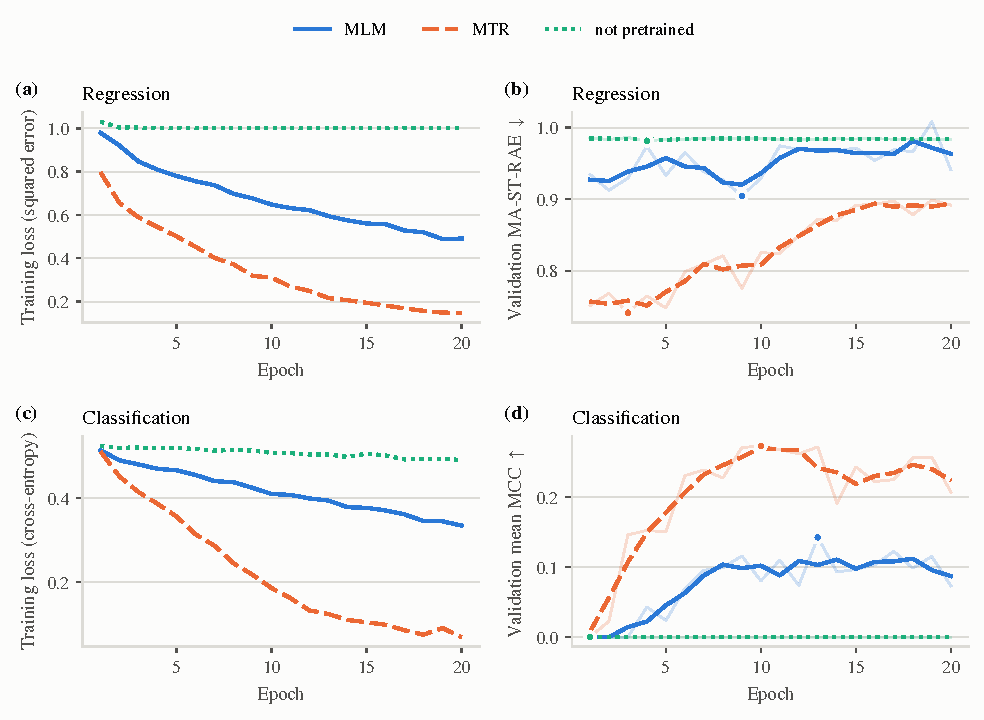
\includegraphics[width=\linewidth]{figuras/fig1_pretraining_objective.pdf}
  \caption{\textbf{Effect of the pretraining objective.} Training loss (a, c) and
  validation score (b, d) per epoch for the two released ChemBERTa-2 checkpoints
  and an untrained control, with pooling fixed to the \textsc{cls} token and the
  encoder fine-tuned. The control uses the same architecture with random weights.
  Validation curves are shown raw (translucent) under a three-epoch rolling mean;
  markers give the epoch selected on validation. MTR reaches both a lower training
  loss and a better validation score than MLM in the two tasks, while the untrained
  control stays at the level of predicting the training mean
  (MA-ST-RAE $\approx 1$) and of calling every molecule negative (MCC $= 0$).}
  \label{fig:pretraining}
\end{figure}

\begin{figure}[t]
  \centering
  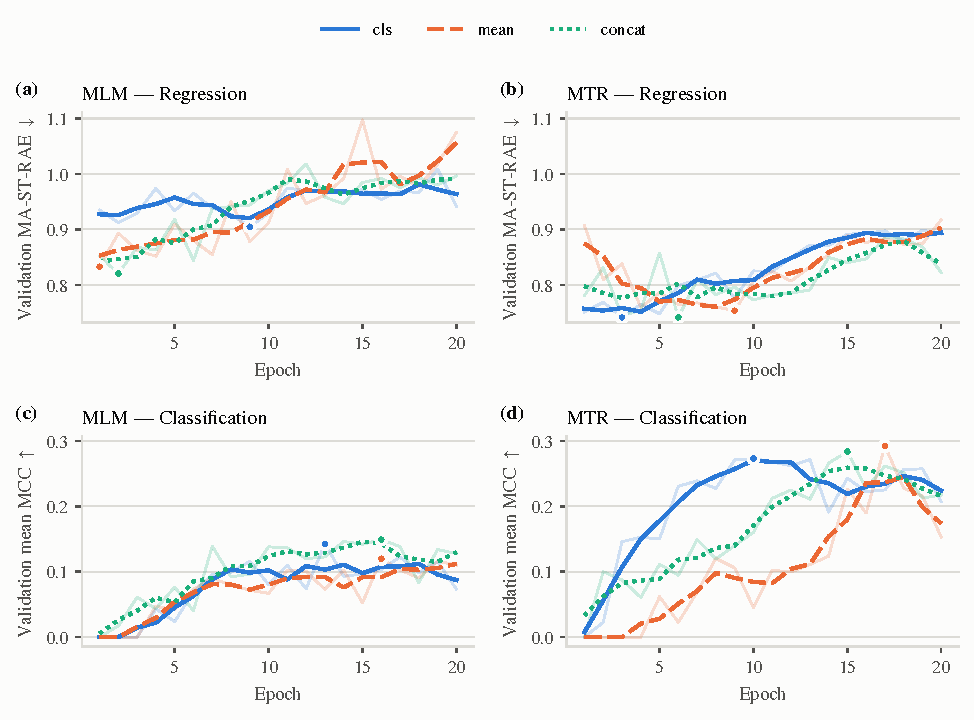
\includegraphics[width=\linewidth]{figuras/fig2_pooling.pdf}
  \caption{\textbf{Effect of the pooling operation, per checkpoint.} Validation
  score per epoch for the three ways of reducing the token sequence to one vector:
  the \textsc{cls} token, the mean over real tokens, and their concatenation. The
  vertical scale is shared within each row so the two checkpoints can be compared
  directly. Pooling matters for MLM, where \textsc{cls} is the weakest option, and
  the three choices are within noise of each other for MTR.}
  \label{fig:pooling}
\end{figure}

\begin{figure}[t]
  \centering
  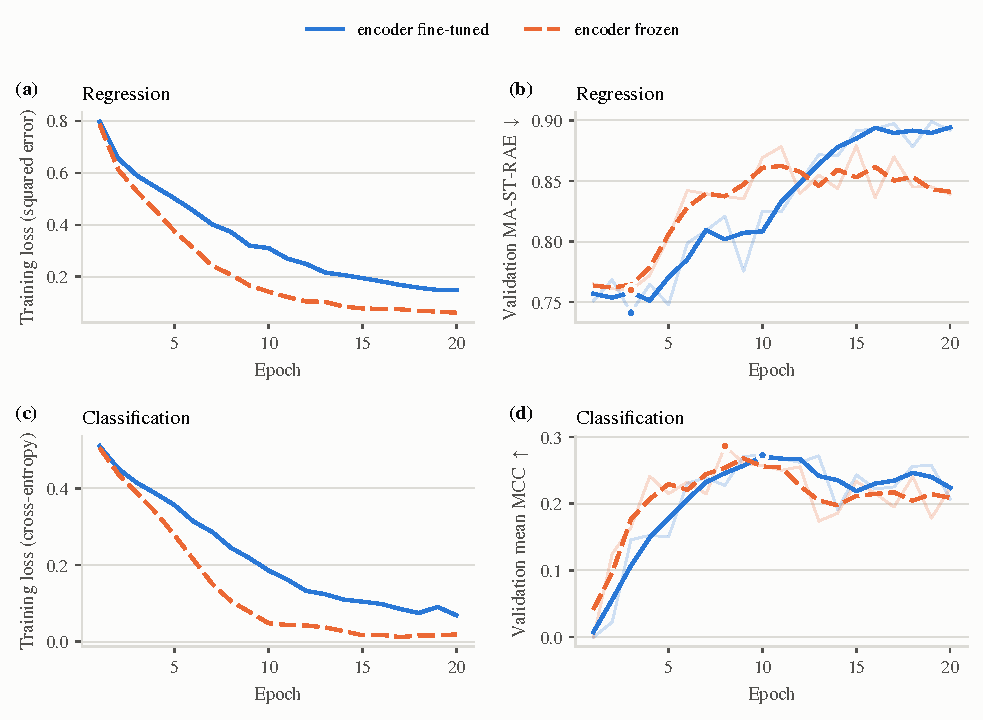
\includegraphics[width=\linewidth]{figuras/fig3_frozen_vs_finetuned.pdf}
  \caption{\textbf{Frozen versus fine-tuned encoder} (MTR checkpoint,
  \textsc{cls} pooling). The frozen run trains the readout head only. Its training
  loss is the lower of the two because freezing the encoder also disables its
  dropout, so the comparison of panels (a) and (c) is not like for like; the
  validation panels (b) and (d) are. The two protocols end within the run-to-run
  spread of each other, at roughly one fifth of the compute.}
  \label{fig:frozen}
\end{figure}

\begin{figure}[t]
  \centering
  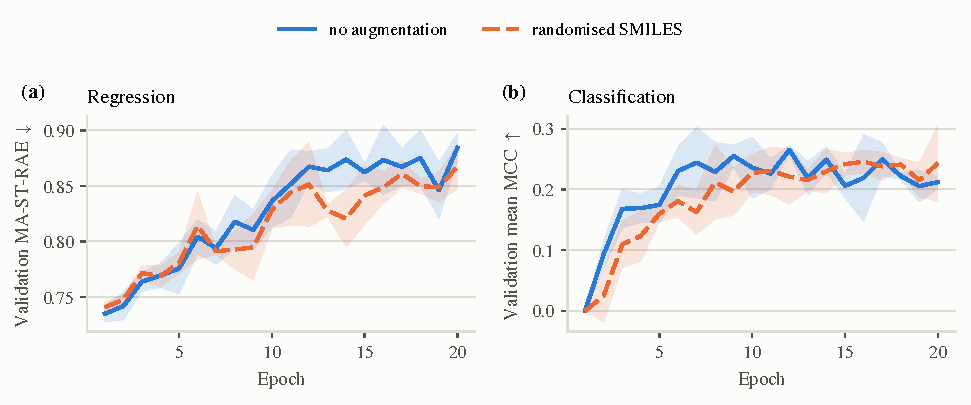
\includegraphics[width=\linewidth]{figuras/fig4_augmentation.pdf}
  \caption{\textbf{SMILES randomisation as data augmentation.} Validation score
  per epoch with and without rewriting each molecule as a different, equally valid
  SMILES string at every epoch; augmentation is applied to the training split only.
  Line: mean of three seeds; band: $\pm$1 s.d. The bands overlap throughout, and at
  the selected epochs the difference is not significant ($p = 0.13$ for regression
  and $p = 0.26$ for classification, two-sided $t$-test, $n = 3$).}
  \label{fig:augmentation}
\end{figure}

\begin{figure}[t]
  \centering
  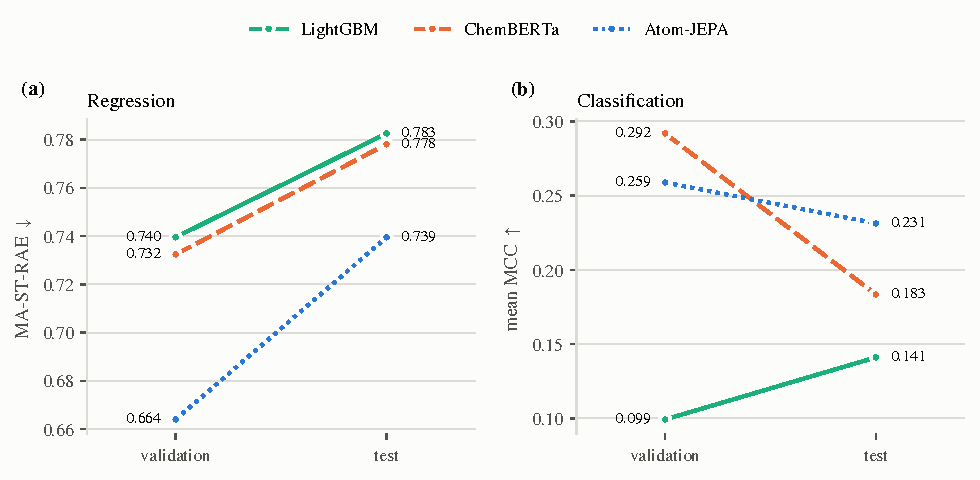
\includegraphics[width=\linewidth]{figuras/fig5_validation_to_test.pdf}
  \caption{\textbf{From validation to test} for the three models, each evaluated
  once on test after its configuration had been fixed on validation. ChemBERTa is
  the mean of three seeds. The ranking is preserved in regression but inverts in
  classification, where ChemBERTa falls 0.108 against 0.028 for Atom-JEPA. The
  ChemBERTa configuration was chosen by comparing some 64 validation runs, whereas
  Atom-JEPA and LightGBM were each run once with default settings, so the
  validation figure is optimistic by an amount the other two do not carry.}
  \label{fig:valtest}
\end{figure}

\begin{figure}[t]
  \centering
  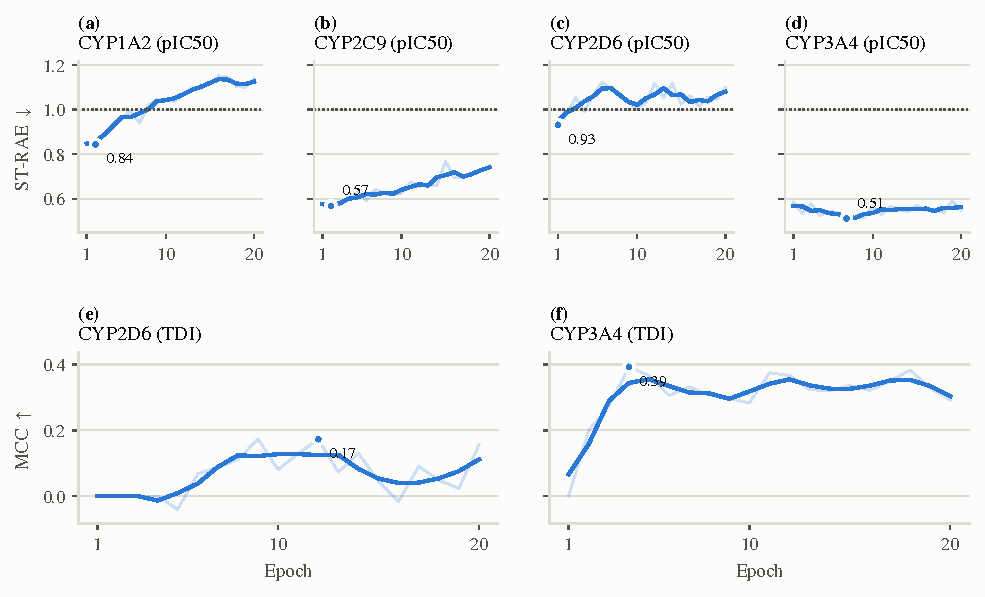
\includegraphics[width=\linewidth]{figuras/fig6_per_endpoint.pdf}
  \caption{\textbf{Per-endpoint behaviour of the selected configuration}
  (MTR, \textsc{cls}, fine-tuned, seed 1): regression (a--d) and classification
  (e--f). The vertical scale is shared within each row; the dotted line marks the
  mean predictor, so any curve above it predicts worse than the training mean.
  Markers give the per-endpoint value at the epoch selected on the macro score.
  The two endpoints with the most labelled molecules, CYP3A4 and CYP2C9, carry the
  result; CYP1A2 and CYP2D6 sit at or above the mean predictor for most of the run.}
  \label{fig:perendpoint}
\end{figure}
